% Enigma Lab · informe final (spec, sección 10): 3 páginas como máximo, 11 pt, una columna.
%
% Compilar:  make report   (latexmk o Tectonic; si no hay LaTeX, sube report/ a Overleaf
% con informe.tex, numbers.tex y la carpeta figuras/).
%
% Todas las cifras entran por numbers.tex (macros \EL…), que make report genera a partir de
% results/summary.json: no escribas números de resultados a mano.
%
% Los párrafos marcados  % REVISAR  son borradores de análisis: reescríbelos con tu voz.
\documentclass[11pt]{article}

\usepackage{iftex}
\ifPDFTeX
  \usepackage[T1]{fontenc}
  \usepackage[utf8]{inputenc}
  \usepackage{lmodern}
\else
  \usepackage{fontspec}
\fi
\usepackage[spanish,es-tabla,es-noshorthands,es-nodecimaldot]{babel}
\usepackage[letterpaper,margin=1.8cm]{geometry}
\usepackage{graphicx}
\usepackage{booktabs}
\usepackage{tabularx}
\usepackage{amsmath}
\usepackage[font=small,labelfont=bf,skip=3pt]{caption}
\usepackage{enumitem}
\usepackage{multicol}
\usepackage{microtype}
\usepackage[hidelinks]{hyperref}

\setlist{nosep,leftmargin=1.2em}
\setlength{\parskip}{0.25em}
\setlength{\parindent}{0pt}
\setlength{\textfloatsep}{8pt plus 2pt minus 2pt}
\setlength{\floatsep}{6pt plus 2pt minus 2pt}
\makeatletter
\renewcommand\section{\@startsection{section}{1}{\z@}{-1.6ex plus -0.5ex}{0.6ex}{\normalfont\large\bfseries}}
\makeatother

% Generado por  make report  (python -m enigma_lab.informe) a partir de
% results/summary.json y los resultados guardados. No lo edites a mano.

\newcommand{\ELalemanLetrasProfundidad}{332}
\newcommand{\ELalemanTrigramasAzar}{357}
\newcommand{\ELalemanTrigramasProfundidad}{254}
\newcommand{\ELanosFuerzaBruta}{5.037}
\newcommand{\ELanosMilMaquinas}{5,04}
\newcommand{\ELataqueCorto}{100}
\newcommand{\ELataqueDiezCorto}{0~\%}
\newcommand{\ELataqueDiezLargo}{25~\%}
\newcommand{\ELataqueLargo}{1.500}
\newcommand{\ELataqueLseis}{314}
\newcommand{\ELataqueMensajes}{864}
\newcommand{\ELataqueN}{24}
\newcommand{\ELataqueOraculoCorto}{29~\%}
\newcommand{\ELataqueOraculoECorto}{46~\%}
\newcommand{\ELataqueSegundos}{1,7}
\newcommand{\ELataqueSeisLargo}{96~\%}
\newcommand{\ELataqueUbicaciones}{1.054.560}
\newcommand{\ELbarrido}{1.054.560}
\newcommand{\ELbitsAnillos}{9,40}
\newcommand{\ELbitsBarrido}{20,01}
\newcommand{\ELbitsConAnillos}{76,51}
\newcommand{\ELbitsOrden}{5,91}
\newcommand{\ELbitsPlugboard}{47,10}
\newcommand{\ELbitsPosiciones}{14,10}
\newcommand{\ELbitsSinAnillos}{67,11}
\newcommand{\ELbrechaSobrepaso}{30,7}
\newcommand{\ELbrechaTotal}{30,9}
\newcommand{\ELcablesClave}{10}
\newcommand{\ELcablesMaximo}{11}
\newcommand{\ELceldasCerca}{15}
\newcommand{\ELceldasTuring}{17}
\newcommand{\ELclavesConAnillos}{$\mathrm{1{,}07}\times10^{23}$}
\newcommand{\ELclavesSinAnillos}{$\mathrm{1{,}59}\times10^{20}$}
\newcommand{\ELcolaDos}{26}
\newcommand{\ELcolaUno}{650}
\newcommand{\ELcolisiones}{650}
\newcommand{\ELcommit}{67e022b}
\newcommand{\ELcribLetras}{250}
\newcommand{\ELcribN}{1.000}
\newcommand{\ELcumpleanos}{157}
\newcommand{\ELcumpleanosP}{50,28~\%}
\newcommand{\ELdecibanNoRepeticion}{\ensuremath{-}0,093}
\newcommand{\ELdecibanRepeticion}{+1,845}
\newcommand{\ELdemoCasos}{60}
\newcommand{\ELdemoExito}{60 de 60}
\newcommand{\ELdemoLetras}{78}
\newcommand{\ELdemoNucleos}{6}
\newcommand{\ELdemoPnoventaycinco}{9,8}
\newcommand{\ELdentroICaleatorio}{10 de 10}
\newcommand{\ELdentroICaleman}{0 de 10}
\newcommand{\ELdentroICkappa}{10 de 10}
\newcommand{\ELderivaAzar}{\ensuremath{-}0,0184}
\newcommand{\ELderivaProfundidad}{+0,0211}
\newcommand{\ELdia}{2026-11-22}
\newcommand{\ELdiagonalFactor}{648}
\newcommand{\ELenSesentaCero}{40.656}
\newcommand{\ELenSesentaDos}{59,4}
\newcommand{\ELenSesentaTres}{6,6}
\newcommand{\ELenSesentaUno}{1.577}
\newcommand{\ELexactoAzar}{1.067,4}
\newcommand{\ELexactoProfundidad}{959,7}
\newcommand{\ELexitoBletchley}{55,0~\%}
\newcommand{\ELexitoRobusto}{98,0~\%}
\newcommand{\ELexitoSinVuelta}{100,0~\%}
\newcommand{\ELfecha}{2026-11-22 17:13 UTC}
\newcommand{\ELfraccionPlugboard}{70,2~\%}
\newcommand{\ELfueraCiclo}{676}
\newcommand{\ELgilloglyDiez}{1.463}
\newcommand{\ELgilloglySeis}{300}
\newcommand{\ELicCifrado}{0,0385}
\newcommand{\ELicCorpusAleman}{0,0757}
\newcommand{\ELicReferencia}{0,0758}
\newcommand{\ELinvolucion}{2.000}
\newcommand{\ELinvoluciones}{$\mathrm{7{,}9}\times10^{12}$}
\newcommand{\ELkappaAleman}{0,0802}
\newcommand{\ELkuhlCaracteristicas}{21.230}
\newcommand{\ELkuhlMayor}{1.771}
\newcommand{\ELkuhlUnicas}{11.466}
\newcommand{\ELmenus}{2.000}
\newcommand{\ELmenusPorCelda}{100}
\newcommand{\ELminutosExperimentos}{30}
\newcommand{\ELmodo}{completo}
\newcommand{\ELparadasCero}{678}
\newcommand{\ELparadasDos}{0,99}
\newcommand{\ELparadasTres}{0,11}
\newcommand{\ELparadasUno}{26,3}
\newcommand{\ELparesBanbu}{2.000}
\newcommand{\ELperiodo}{16.900}
\newcommand{\ELpermutaciones}{$\mathrm{4}\times10^{26}$}
\newcommand{\ELporLazo}{26}
\newcommand{\ELpropiedadesClaves}{2.000}
\newcommand{\ELpropiedadesLetras}{200.000}
\newcommand{\ELpuntosFijos}{0}
\newcommand{\ELpyenigmaCasos}{10.000}
\newcommand{\ELpyenigmaCoinciden}{10.000}
\newcommand{\ELpyenigmaICalto}{100~\%}
\newcommand{\ELpyenigmaICbajo}{99,96~\%}
\newcommand{\ELpyenigmaLetras}{1.007.710}
\newcommand{\ELrejCaracteristicaMensajes}{49,1}
\newcommand{\ELrejCaracteristicas}{21.225}
\newcommand{\ELrejConfiguraciones}{105.456}
\newcommand{\ELrejDias}{4.000}
\newcommand{\ELrejEncontrada}{75,4~\%}
\newcommand{\ELrejMayor}{1.728}
\newcommand{\ELrejPermutacion}{60,7}
\newcommand{\ELrejTodas}{128,0}
\newcommand{\ELrejTodasTeoria}{127,1}
\newcommand{\ELrejUnicas}{11.578}
\newcommand{\ELrejVuelta}{26,0~\%}
\newcommand{\ELrobustoParadas}{10,9}
\newcommand{\ELrobustoTiempo}{12,0}
\newcommand{\ELsegundosOrden}{0,008}
\newcommand{\ELsegundosOrdenRobusto}{0,11}
\newcommand{\ELsemilla}{2026}
\newcommand{\ELsimAzar}{1.090}
\newcommand{\ELsimAzarAlto}{1.120}
\newcommand{\ELsimAzarBajo}{1.061}
\newcommand{\ELsimProfundidad}{983}
\newcommand{\ELsimProfundidadAlto}{1.012}
\newcommand{\ELsimProfundidadBajo}{954}
\newcommand{\ELsinDiagonalCero}{17.575}
\newcommand{\ELsinDiagonalDos}{729}
\newcommand{\ELsinDiagonalTres}{27,4}
\newcommand{\ELsinDiagonalUno}{17.040}
\newcommand{\ELsinPuntoFijoCien}{1,98~\%}
\newcommand{\ELsobrepasoArriba}{0,65}
\newcommand{\ELsobreviveCincuenta}{14,1~\%}
\newcommand{\ELsobreviveTrece}{60,1~\%}
\newcommand{\ELsobreviveTreceAleman}{61,6~\%}
\newcommand{\ELsobreviveTreceAlto}{60,3~\%}
\newcommand{\ELsobreviveTreceBajo}{59,9~\%}
\newcommand{\ELtasaCorpus}{0,0802}
\newcommand{\ELtasaCorpusInversa}{12,5}
\newcommand{\ELteoriaKappaTrece}{61,4~\%}
\newcommand{\ELteoriaTrece}{60,1~\%}
\newcommand{\ELturingCero}{820}
\newcommand{\ELturingDos}{1,2}
\newcommand{\ELturingSesentaCero}{49.200}
\newcommand{\ELturingSesentaDos}{72}
\newcommand{\ELturingSesentaTres}{2,4}
\newcommand{\ELturingSesentaUno}{1.860}
\newcommand{\ELturingTres}{0,04}
\newcommand{\ELturingUno}{31}
\newcommand{\ELumbral}{19,96}
\newcommand{\ELvectoresOk}{9}
\newcommand{\ELvectoresTotal}{9}
\newcommand{\ELvuelta}{45,0~\%}
\newcommand{\ELwaldAzar}{1.062}
\newcommand{\ELwaldProfundidad}{929}


\begin{document}

\begin{center}
  {\Large\bfseries Romper Enigma: simulación y criptoanálisis estadístico\\[2pt]
  de Enigma~I, la Bombe de Turing-Welchman y el Banburismus}\\[6pt]
  Carlos Daniel Guarin Ortiz · Criptografía · Universidad Nacional de Colombia · 2026\\[2pt]
  {\small Código, app y datos: repositorio Enigma Lab % REVISAR: agrega aquí el enlace del repositorio remoto
  · cifras de la corrida en modo \ELmodo{} del \ELfecha{} (commit \texttt{\ELcommit}, semilla \ELsemilla)}
\end{center}

\section{Objetivo}

¿Por qué se rompió un cifrado con \ELclavesSinAnillos{} claves (\ELbitsSinAnillos{} bits:
Enigma~I con \ELcablesClave{} cables, sin contar los anillos), y cuánta información necesita
cada ataque? La hipótesis es «divide y vencerás»: el plugboard aporta \ELbitsPlugboard{} de esos
bits (el \ELfraccionPlugboard), pero la estructura de la máquina permite apartarlo, y la Bombe
de Turing-Welchman solo recorre 60 órdenes de rotores por 17.576 posiciones: \ELbarrido{}
configuraciones, \ELbitsBarrido{} bits. El objetivo fue reproducir en software los ataques
históricos y medir con simulación Monte Carlo cuánto cuestan y con qué probabilidad funcionan,
comparando cada resultado con las cifras de Turing y de la literatura.

\section{Contexto en el curso}

% REVISAR
Enigma reúne los temas del curso: el cableado se conocía desde 1932, así que solo la clave era
secreta (Kerckhoffs); es un cifrado de flujo de permutaciones cuyo odómetro se repite cada
\ELperiodo{} letras; los cribs son texto plano conocido; que ninguna letra se cifre a sí misma
es un distinguidor perfecto; y los mensajes «en profundidad» son la reutilización del flujo que
hoy evita un nonce único. Y deja la lección del costo del mejor ataque: \ELbitsSinAnillos{} bits
separables valen mucho menos, como el doble DES ante el encuentro a medio camino.

\section{Método}

Todo está en Python 3.12 (NumPy, Numba, pandas, SciPy y statsmodels), con una app en Streamlit
que hace de demostración en vivo; la lógica de Enigma existe una sola vez, en el paquete
\texttt{enigma\_lab}, y las animaciones solo dibujan trazas calculadas en Python.
\begin{itemize}
  \item \textbf{Simulador.} Enigma~I, M3 y M4 con anillos, plugboard y doble paso, más una
  versión vectorizada para el Monte Carlo. Se validó (E1) con los vectores publicados, contra
  py-enigma (una implementación independiente) en \ELpyenigmaCasos{} claves y mensajes
  aleatorios, a mano con CyberChef y con pruebas de propiedades.
  \item \textbf{Espacio de claves (E2).} Conteo exacto con enteros:
  $N(k)=26!/\bigl((26-2k)!\,k!\,2^k\bigr)$ formas de poner $k$ cables.
  \item \textbf{Cribs (E4).} \ELcribN{} mensajes de \ELcribLetras{} letras por longitud $L$
  (5 a 50), con el crib en una posición al azar, en texto aleatorio y en alemán real (Fontane y
  Kafka, de Project Gutenberg, con la X como separador): fracción de alineaciones falsas sin
  conflictos.
  \item \textbf{Bombe (E5).} Modelo eléctrico de 26 cables por 26 hilos: cada arista $(a,b,i)$
  del menú une el hilo $u$ del cable $a$ con el hilo $S_i(u)$ del cable $b$, y el diagonal board
  une el hilo $u$ de $a$ con el hilo $a$ de $u$. La componente encendida se calcula con
  union-find en Numba; hay parada si el cable de prueba no queda entero encendido. Se barrió el
  orden verdadero de \ELmenusPorCelda{} menús por celda (8 a 16 letras, 0 a 3 lazos), con y sin
  diagonal board; un verificador completa luego el plugboard y los anillos.
  \item \textbf{Banburismus (E6).} Pares en profundidad cifrados con la máquina real. Cada
  columna suma $10\log_{10}$ del cociente de verosimilitudes (decibanes) con tasas de repetición
  1/17 y 1/26: \ELdecibanRepeticion{} dB si repite y \ELdecibanNoRepeticion{} dB si no. La
  prueba secuencial de Wald decide con $\alpha=\beta=1~\%$ (umbrales de
  $\pm$\ELumbral{}~dB), con \ELparesBanbu{} pares por condición y, para letras sueltas, un
  cálculo exacto del tiempo de parada.
\end{itemize}
Semilla \ELsemilla; intervalos de Wilson para proporciones y normales para medias.
\texttt{make reproduce} repite los seis experimentos en unos \ELminutosExperimentos{} minutos.

\section{Resultados}

\begin{table}[t]
  \centering\small
  \caption{Validación del simulador (E1) y espacio de claves de Enigma~I con
  \ELcablesClave{} cables (E2).}\label{tab:validacion}
  \begin{tabularx}{\textwidth}{@{}Xl@{}}
    \toprule
    Prueba o cantidad & Resultado \\
    \midrule
    Vectores publicados (BDZGO, EWTYX, py-enigma, U-264 y los de las diapositivas) &
      \ELvectoresOk{} de \ELvectoresTotal \\
    py-enigma con claves y mensajes aleatorios (\ELpyenigmaLetras{} letras, 0 a 10 cables) &
      \ELpyenigmaCoinciden{} de \ELpyenigmaCasos{} (IC 95~\%: \ELpyenigmaICbajo--100~\%) \\
    Puntos fijos en \ELpropiedadesLetras{} letras · cifrar dos veces devuelve el texto &
      \ELpuntosFijos{} · \ELinvolucion{} de \ELpropiedadesClaves{} claves \\
    Periodo del odómetro I-II-III (posiciones fuera del ciclo) & \ELperiodo{} (\ELfueraCiclo) \\
    \midrule
    Claves sin anillos · con anillos &
      \ELclavesSinAnillos{} (\ELbitsSinAnillos{} bits) · \ELclavesConAnillos{} (\ELbitsConAnillos{} bits) \\
    Bits del orden · las posiciones · los anillos · el plugboard &
      \ELbitsOrden{} · \ELbitsPosiciones{} · \ELbitsAnillos{} · \ELbitsPlugboard \\
    Barrido de la Bombe (60 órdenes $\times$ 17.576 posiciones) &
      \ELbarrido{} (\ELbitsBarrido{} bits) \\
    Fuerza bruta a $10^9$ claves por segundo (sin anillos) & \ELanosFuerzaBruta{} años \\
    \bottomrule
  \end{tabularx}
\end{table}

\textbf{Validación (tabla~\ref{tab:validacion}).} El simulador coincide con py-enigma y con todos
los vectores publicados. \textbf{Cribs (figura~\ref{fig:e4}).} Con texto aleatorio, $(25/26)^L$ cae dentro del IC 95~\% en
\ELdentroICaleatorio{} longitudes: con 13 letras sobrevive el \ELsobreviveTrece{} de las
alineaciones falsas (IC \ELsobreviveTreceBajo--\ELsobreviveTreceAlto), y con 50, el
\ELsobreviveCincuenta. Con alemán real sobreviven algo más (\ELsobreviveTreceAleman{} con 13
letras) y $(25/26)^L$ queda fuera del IC en las 10 longitudes; la corrección
$\bigl(1-(1-\kappa)/25\bigr)^L$, con $\kappa=$~\ELkappaAleman{} medido en el corpus, queda dentro
en \ELdentroICkappa.

\begin{figure}[t]
  \centering
  \begin{minipage}[t]{0.495\textwidth}
    \centering
    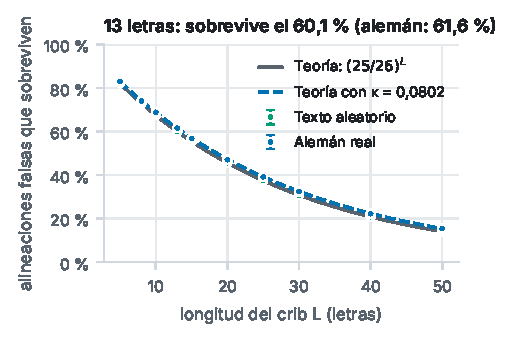
\includegraphics[width=\linewidth]{figuras/e4_cribs.pdf}
    \caption{E4: alineaciones falsas que sobreviven al crib (media e IC 95~\% de \ELcribN{}
    mensajes por longitud) frente a $(25/26)^L$ y a la teoría con el IC del alemán.}\label{fig:e4}
  \end{minipage}\hfill
  \begin{minipage}[t]{0.495\textwidth}
    \centering
    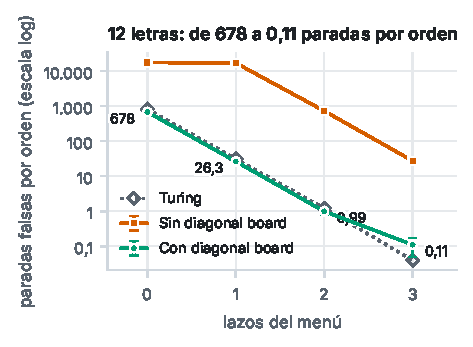
\includegraphics[width=\linewidth]{figuras/e5_bombe.pdf}
    \caption{E5: paradas falsas por orden de rotores con 12 letras en el menú (modo Bletchley,
    \ELmenusPorCelda{} menús por punto, IC 95~\%) frente a la estimación de Turing.}\label{fig:e5}
  \end{minipage}
\end{figure}

\textbf{Bombe (figura~\ref{fig:e5}).} Con 12 letras y diagonal board, las paradas falsas por orden
con 0 a 3 lazos son \ELparadasCero{} · \ELparadasUno{} · \ELparadasDos{} · \ELparadasTres{}
(Turing: \ELturingCero{} · \ELturingUno{} · \ELturingDos{} · \ELturingTres). En \ELceldasCerca{} de
las \ELceldasTuring{} celdas de su tabla con valor exacto, lo medido queda entre la mitad y el
doble de su estimación. Sin diagonal board hay \ELdiagonalFactor{} veces más paradas con un lazo
(\ELsinDiagonalUno{} por orden). El rotor central se movió dentro del crib en el \ELvuelta{} de
los menús, y ahí el modo Bletchley pierde la parada verdadera (éxito \ELexitoBletchley); el modo
robusto la encuentra en el \ELexitoRobusto{} con \ELrobustoTiempo{} veces el tiempo. En la app,
la demo con WETTERBERICHT y los 60 órdenes rompe \ELdemoExito{} cifrados de \ELdemoLetras{}
letras, con un p95 de \ELdemoPnoventaycinco~s (escritorio de \ELdemoNucleos{} núcleos).

\textbf{Banburismus (figura~\ref{fig:e6}).} Con la tasa 1/17, la profundidad se confirma en
\ELsimProfundidad{} letras en promedio (IC \ELsimProfundidadBajo--\ELsimProfundidadAlto) y se
descarta en \ELsimAzar; la aproximación de Wald da \ELwaldProfundidad{} y \ELwaldAzar, y el
cálculo exacto, \ELexactoProfundidad{} y \ELexactoAzar. Con alemán real y los mismos pesos de
Turing bastan \ELalemanLetrasProfundidad{} letras, y \ELalemanTrigramasProfundidad{} puntuando
bigramas y trigramas.

\begin{figure}[t]
  \centering
  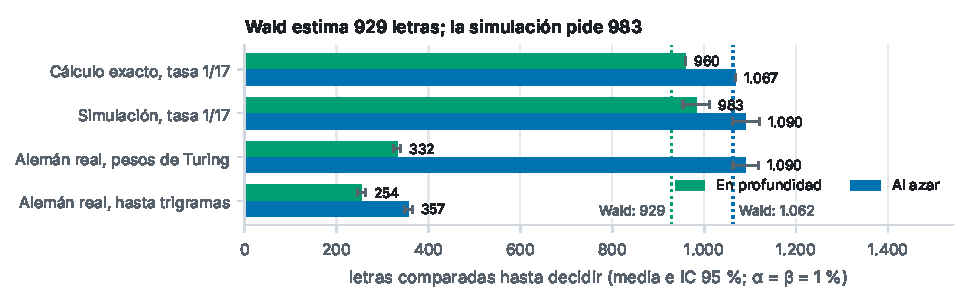
\includegraphics[width=\textwidth]{figuras/e6_sprt.pdf}
  \caption{E6: letras hasta que el SPRT decide ($\alpha=\beta=1~\%$), media e IC 95~\% de
  \ELparesBanbu{} pares por condición. Las líneas punteadas son la aproximación de Wald con letras
  sueltas.}\label{fig:e6}
\end{figure}

\section{Análisis y lecciones}

% REVISAR
\textbf{Divide y vencerás.} El experimento confirma la hipótesis: la Bombe no necesita los
\ELbitsPlugboard{} bits del plugboard porque prueba hipótesis sobre un solo stecker y deja que
el menú propague las consecuencias; recorre \ELbitsBarrido{} bits y no \ELbitsSinAnillos.

% REVISAR
\textbf{Cribs y menús.} El filtro del crib es barato pero débil: con 13 letras deja pasar el
\ELsobreviveTrece{} de las posiciones falsas; con alemán real, algo más, por su índice de
coincidencia. La fuerza está en los lazos: hasta 2, cada uno divide las paradas por unas 26,
porque la letra supuesta debe ser un punto fijo de la permutación del lazo. Con 3 lazos medimos
\ELparadasTres{} frente a \ELturingTres{} de Turing: son muy pocas paradas, pero el IC no incluye
su valor y lo reportamos como diferencia. Sin diagonal board, un menú sin lazos no descarta casi
nada.

% REVISAR
\textbf{Wald y el sobrepaso.} La aproximación de Wald supone que la prueba se detiene justo en el
umbral; en realidad lo pasa (en promedio \ELsobrepasoArriba~dB arriba), y eso explica
\ELbrechaSobrepaso{} de las \ELbrechaTotal{} letras de diferencia en profundidad. Con texto real
la profundidad se confirma en un tercio de las letras porque el alemán literario repite 1 de cada
\ELtasaCorpusInversa{} letras, más que el 1 de cada 17 del tráfico naval.

% REVISAR
\textbf{Lecciones y límites.} El tamaño de la clave no es la seguridad: cuenta el mejor ataque;
cualquier sesgo es un distinguidor y reutilizar un nonce deja dos mensajes en profundidad. No se
hizo la fase opcional (el catálogo de Rejewski y el ataque moderno de solo texto cifrado de
Gillogly y de Ostwald y Weierud): la presentación solo cita la literatura. El corpus es
literario, no naval, y los tiempos son de un escritorio, no del portátil de la presentación.

\section*{Referencias}
{\footnotesize
\begin{multicols}{2}
\begin{enumerate}[label={[\arabic*]},leftmargin=2em,itemsep=0pt]
  \item A.~M.~Turing (c.~1941--42). \emph{The Applications of Probability to Cryptography}.
  The National Archives, HW 25/37. \url{https://arxiv.org/abs/1505.04714}
  \item M.~Rejewski (1980). An application of the theory of permutations in breaking the Enigma
  cipher. \emph{Applicationes Mathematicae} 16(4), 543--559.
  \item J.~Wilcox (2006). \emph{Solving the Enigma: History of the Cryptanalytic Bombe}. NSA,
  Center for Cryptologic History.
  \item I.~J.~Good (1979). A.~M.~Turing's statistical work in World War II. \emph{Biometrika}
  66(2), 393--396.
  \item A.~Wald (1945). Sequential tests of statistical hypotheses. \emph{The Annals of
  Mathematical Statistics} 16(2), 117--186.
  \item A.~Kuhl (2007). Rejewski's catalog. \emph{Cryptologia} 31(4), 326--331.
  \item J.~J.~Gillogly (1995). Ciphertext-only cryptanalysis of Enigma. \emph{Cryptologia}
  19(4), 405--413.
  \item O.~Ostwald y F.~Weierud (2017). Modern breaking of Enigma ciphertexts.
  \emph{Cryptologia} 41(5), 395--421.
  \item J.~Weinbaum. \emph{Action This Day} (tesis de maestría, Dartmouth College).
  \item K.~Pommerening. Notas de criptología clásica: Enigma. Universidad de Mainz.
  \item Wikipedia: «Bombe» (tabla de paradas de Turing, revisión 1385546242), «Banburismus»
  (revisión 1372577431) y «Enigma rotor details» (revisión 1275803743).
  \item D.~Rijmenants. \emph{The M4 Project} (mensaje del U-264, 1942). Cipher Machines and
  Cryptology.
  \item B.~Neal. py-enigma 1.0.2; GCHQ, CyberChef (operaciones Enigma y Bombe).
  \item Project Gutenberg: T.~Fontane, \emph{Effi Briest}; F.~Kafka, \emph{Die Verwandlung}.
\end{enumerate}
\end{multicols}
}

\end{document}
